\begin{figure}[tb]
  \begin{subfigure}[t]{0.35\linewidth}
    \centering
    \caption{}
    \label{subfig:performance-cifar10-3c3d-cuda_main_1}

    \vspace{-\baselineskip}
    \begin{normalsize}
      $N_{\text{crit}}$ (eigenvalues)
    \end{normalsize}
    \vspace{0.15\baselineskip}

    \begin{normalsize}
      \begin{tabular}{lll}
    \toprule
    $_{\text{\tiny{\ggn}}}$$^{\text{\tiny{Data}}}$ & mb & sub \\
    \midrule
    exact & 208
              & 727 \\
    mc   & 1055
              & 1816 \\
    \bottomrule
\end{tabular}
    \end{normalsize}

    \vspace{\baselineskip}

    \begin{normalsize}
      $N_{\text{crit}}$ (top eigenpair)
    \end{normalsize}
    \vspace{0.15\baselineskip}

    \begin{normalsize}
      \begin{tabular}{lll}
    \toprule
    $_{\text{\tiny{\ggn}}}$$^{\text{\tiny{Data}}}$ & mb & sub \\
    \midrule
    exact & 208
              & 727 \\
    mc   & 1055
              & 1816 \\
    \bottomrule
\end{tabular}
    \end{normalsize}

    \vspace{3.6\baselineskip}

  \end{subfigure}
  \begin{subfigure}[t]{0.64\linewidth}
    \centering
    \caption{}
    \label{subfig:performance-cifar10-3c3d-cuda_main_2}

    \vspace{-1.5\baselineskip}

    % load "performancedefault" style
    % defines the pgfplots style "performancedefault"
\pgfkeys{/pgfplots/performancedefault/.style={
    width=1.04\linewidth,
    height=\goldenRatioInv*1.04\linewidth,
    every axis plot/.append style={line width = 1.2pt},
    every axis plot post/.append style={
      mark size=2, mark options={opacity=0.9, solid, line width = 1pt}
    },
    tick pos = left,
    xmajorticks = true,
    ymajorticks = true,
    ylabel near ticks,
    xlabel near ticks,
    xtick align = inside,
    ytick align = inside,
    legend cell align = left,
    legend columns = 3,
    % legend pos = north east,
    legend style = {
      fill opacity = 0.9,
      text opacity = 1,
      font = \small,
      at={(1, 1.025)},
      anchor=south east,
    },
    xticklabel style = {font = \small, inner xsep = 0ex},
    xlabel style = {font = \small},
    axis line style = {black},
    yticklabel style = {font = \small, inner ysep = 0ex},
    ylabel style = {font = \small, inner ysep = 0ex},
    title style = {font = \small, inner ysep = 0ex, yshift = -0.75ex},
    grid = major,
    grid style = {dashed},
    title = {},
  }
}
%%% Local Variables:
%%% mode: latex
%%% TeX-master: "../main"
%%% End:

    % customize "zmystyle" as you wish
    \pgfkeys{/pgfplots/zmystyle/.style={performancedefault, height=0.5\linewidth}}
    % This file was created by tikzplotlib v0.9.7.
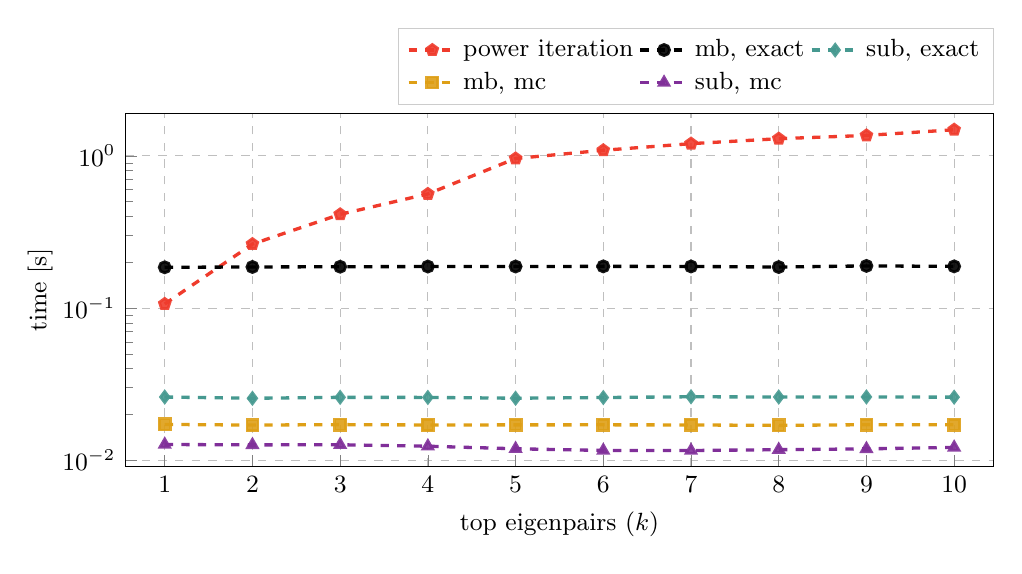
\begin{tikzpicture}

\definecolor{color0}{rgb}{0.937254901960784,0.231372549019608,0.172549019607843}
\definecolor{color1}{rgb}{0.274509803921569,0.6,0.564705882352941}
\definecolor{color2}{rgb}{0.870588235294118,0.623529411764706,0.0862745098039216}
\definecolor{color3}{rgb}{0.501960784313725,0.184313725490196,0.6}

\begin{axis}[
axis line style={white!80!black},
legend style={fill opacity=0.8, draw opacity=1, text opacity=1, at={(0.03,0.97)}, anchor=north west, draw=white!80!black},
tick pos=left,
title={cifar10\_3c3d, N=128, cuda, one\_group},
xlabel={top eigenpairs (\(\displaystyle k\))},
xmin=0.55, xmax=10.45,
ylabel={time [s]},
ymin=0.00910443848057122, ymax=1.89239674986061,
ymode=log,
zmystyle
]
\addplot [, color0, dashed, mark=pentagon*, mark size=3, mark options={solid}]
table {%
1 0.10646684000676
2 0.263332082999113
3 0.41296657500061
4 0.562371585998335
5 0.961040356996818
6 1.08828064100089
7 1.20301098700293
8 1.29626815899974
9 1.36217651501647
10 1.48477111599641
};
\addlegendentry{power iteration}
\addplot [, black, dashed, mark=*, mark size=3, mark options={solid}]
table {%
1 0.185383651005395
2 0.186310245997447
3 0.186981072998606
4 0.187526319001336
5 0.18765962299949
6 0.18803448399558
7 0.187778580999293
8 0.186061766995408
9 0.189352801004134
10 0.188033979997272
};
\addlegendentry{mb, exact}
\addplot [, color1, dashed, mark=diamond*, mark size=3, mark options={solid}]
table {%
1 0.0260587410011794
2 0.0255732080040616
3 0.0259397419940797
4 0.0259047899962752
5 0.0255934300002991
6 0.0258599759981735
7 0.0261660430041957
8 0.02605828599917
9 0.0260880819987506
10 0.0260066910050227
};
\addlegendentry{sub, exact}
\addplot [, color2, dashed, mark=square*, mark size=3, mark options={solid}]
table {%
1 0.0172249570023268
2 0.0170504369962146
3 0.017168151003716
4 0.0170781389970216
5 0.0171006899981876
6 0.0171182029953343
7 0.0170811919961125
8 0.0169726210006047
9 0.017144368001027
10 0.0171162970000296
};
\addlegendentry{mb, mc}
\addplot [, color3, dashed, mark=triangle*, mark size=3, mark options={solid,rotate=180}]
table {%
1 0.0127098220036714
2 0.0126403089961968
3 0.0126599400027771
4 0.0123849169976893
5 0.011915481001779
6 0.0116139689998818
7 0.0116039499989711
8 0.0117499150001095
9 0.0118982629937818
10 0.0121629770001164
};
\addlegendentry{sub, mc}
\end{axis}

\end{tikzpicture}

  \end{subfigure}

  \vspace{-7ex}
  \caption{\textbf{GPU memory and run time performance:}
  Performance measurements for the
  \threecthreed architecture ($D = 895,\!210$)
  on \cifarten ($C=10$).
  \textbf{(a)} Critical batch sizes $N_{\text{crit}}$
    for computing eigenvalues and the top eigenpair.
    \textbf{(b)} Run time comparison with a power iteration for extracting
    the $k$ leading eigenpairs using a batch of size $N=128$.
  }
  \label{fig:performance-cifar10-3c3d-cuda_main}
\end{figure}

%%% Local Variables:
%%% mode: latex
%%% TeX-master: "../main"
%%% End:
